\section{Content \& Digital Preservation}
The information age enables us to produce, transfer and share massive volumes of data freely in an easy fashion. Scientists all over the world conduct complex research experiments and simulations that produce such an enormous amount of information that was unimaginable just a couple of decades ago. In Microsoft Research's book Jim Gray gives a simple example of the order of magnitude of data volume that is going to be produced. The Large Synoptic Survey Telescope\footnote{http://www.lsst.org/lsst/about} will produce around 1.3 petabytes of information only it its first year of operation, which is more than any other telescope in history has produced \cite{Gray:2009:fourthparadigm}.

The World Wide Web has certainly played an important role as a catalyst of this data growth. In order to put this fact into perspective, Intel\textsuperscript{\copyright}\footnote{http://www.intel.com/} has created a famous Infographic presented in figure \ref{fig:intel_oneminute_internet}
As it becomes easier and cheaper to create, edit, manipulate, store and share large amounts of digital objects, people often grow unaware of the problems that arise with the digital content they create.

A single sheet of paper, put in a normal environment, can easily endure a number of decades and will most likely still be readable and accessible. A digital object, a file that contains the exact same content, often does not stand a chance of living through the next decade. Hardware failures, software obsolescence, changed environments, lack of backup copies are just a small set of examples of what may occur to digital objects and render a user unable to access them again.

Digital Preservation is aiming to preserve digital content through the years and make it findable, accessible, readable and understandable for periods of time which often surpass the lifetime of hardware and software components \cite{DBLP:journals/dlib/RosenthalRLRM05}. In the last years, a growing awareness of digital preservation problems is seen throughout scientific communities, memory institutions and business enterprises. These create solutions and follow different approaches and apply specific workflows on content in order to tackle many problems on different levels.

Currently, content holding institutions possess huge amounts of data. Web Archives for example crawl and store web sites and related content, such as images, video, style sheet files, etc. National and state archives use digital repositories to preserve their content. However, crawling and storing the bits and bytes represents only one step towards preserving all this content.

Regardless of the origin of the content (web archive, scientific data, personal audio and video collections, etc.), preservation planning has to be done in order to be able to identify and apply the most meaningful course of action and thus ensure the long-term safety and accessibility of each object that was stored. And since content and the environments which we use to manage it are continuously evolving, this process has to be repeated on a regular basis.

\begin{figure}[hb]
\begin{center}
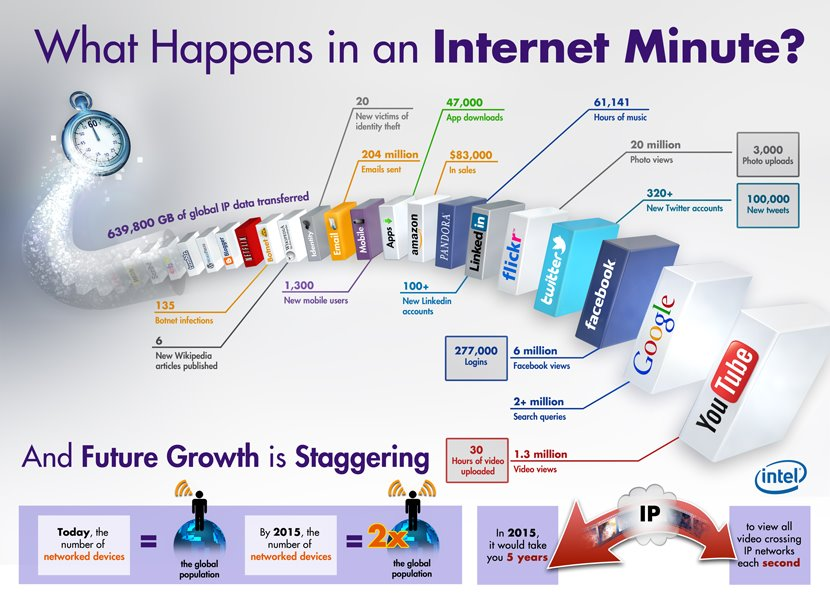
\includegraphics[width=6in]{figures/introduction/intel_oneminute_internet.jpg}
\caption{What happens in an internet minute. (An infographic by Intel\textsuperscript{\copyright})}
\label{fig:intel_oneminute_internet}
\end{center}
\end{figure}

\section{Motivation}
% automation and its importance.
% concetrate on collection profiling
% why is it important to know what do we have
% in the collections.
Due to the fast growth and scale of data, the need of automation support in digital preservation processes arises. In order to conduct preservation planning effectively, one has to undertake a well-defined process consisting of numerous steps \cite{Becker:2009fk}. Very important part of this process is the definition of the content that has to be preserved and the representative sample selection. 

The validity and effectiveness of the planning process is highly dependent on a content profile because it defines the scope of the produced plan. A profile defines the content of a collection in terms of its meta data and properties. This meta data plays an important role when preserving digital objects as it not only carries important information about the objects themselves, but also about their structure. Such information provides hints about the digital objects and their type and helps experts decide the best course of action regarding the long-term accesability and preservation of data. A profile also defines a set of sample objects, that are representative to the whole collection of objects. The selected samples provide the basis for the experiments based on which potential courses of action, called preservation alternatives are evaluated. This means that enough valid meta information and knowledge about the content has to be obtained so that only proper alternatives can be chosen. In order to achieve this goal, some very important and necessary steps that provide valuable input to planning have to be undergone. These are currently not always done efficiently, if done at all. For example, the content has to be characterized and all the meta data that is extracted has to be aggregated and analyzed before all potential preservation action alternatives can be found and evaluated. Based on this analysis the content that is to be preserved can be split up into homogeneous sub-collections with similar characteristics and significant properties. Furthermore, such an aggregation of the similarities between different parts of the content can enable more efficient stratification of representative samples in an automatic fashion.

%Based on these and on objective trees defined in another step of the process the most effective preservation action is chosen.
%cite objective tree and representatives.

The presevation planning process is currently done semi-automatically and needs much input regarding the content profile from a preservation expert. Due to the scale of the data a preservation expert often does not have a specific overview of the content profile, but rather high-level knowledge, such as ``The collection consists of 1 million audio files''. It seems that many parts of this process, from characterization to plan deployment and execution, can be automated or at least enhanced by machine processes. Also support for large-scale processing and analysis can be provided by distributed architectures and state of the art algorithms. If this is achieved the effect will be much more valuable than the sum of its parts for the Digital Preservation community.

Nonetheless, the current state of the art does not specify a concrete and well-defined way of how content profiling should be done and what information it should aggregate. What is more, there are almost no evaluation possibilities of the results that characterization tools offer. Some tools try to give confidence level, which is a first step towards such a validation, however it is not enough. A simple example of such uncertainties is character set encoding of html files. Many files specify a UTF-8 encoding, however the real encoding used in the file is different. Some tools are able to detect this, whereas others just report the declared encoding. This is only one of many examples of such uncertainties that arise due to missing quality assurance steps during the characterization process. Such seemingly minor pecularities can cause huge impact on the chosen preservation alternative and thus on the final result of the preserved content. The ability to detect them on a larger scale, to find out subtleties and nuances between different objects in a collection and to select valid representative objects will greatly enhance the preservation planning process.

Thus, a specific way of aggregating large amounts of meta data and its multidimensional representation would be of great value. Only with such a content profile efficient preservation planning can be achieved.

\section{Problem Statement}
Very often collection and content profiling is done on a very high level, that
is often insufficient for a planning process, especially if this process is to be fully automated.
The current state of the art of content profiling in preservation plans is creating a short description, written by a preservation expert. These descriptions are usualy a very high level assertions, such as: ``The collection contains about 2 million TIFF files''. The profile also contains simple metrics, such as (approximate) collection size, and number of elements as well as the formats identified in the collection. 
These measurements are important but are not the only ones needed for the creation of an efficient preservation plan.
For example, the information about the size of the whole collection is not enough. Other size related measures, such as the overall size of all files in a collection that have a specific format, or the average size of files with a mime type 'text/plain' can be much more significant and helpful in a preservation planning process. Another example where simple measures are not enough are the formats within a collection. In cases of heterogeneous content the distribution of the formats in combination of some other property can turn out to be very helpful for analysis and comprehension of the content. Moreover, in cases of format-homogeneous collections the file format alone will play only a minor role. Combining them with other properties such as the creation date or the creating application could however give deeper insight into the collection.
These are only a few of the examples of multi dimensional characteristics that could turn out to be important in content profiling. However, there are many more that will play different role from case to case.

Furthermore, the creation of a plan has very specific requirements. For example, it needs a small subset of the collection in order to conduct some experiments over it. Based on the results, recommendations and decisions about the preservation actions of the whole collection are produced. Thus the choice of a representative collection subset is a very important process, that is unfortunately often taken lightly, e.g. done randomly or done based on a very shallow analysis. Besides of the manual and random choice of samples in current preservation practices their integration within the planning process is also done manually (either by file upload or manual filling of the related sample information).

Currently, there is no tool that meets these planning requirements and tries to tackle and solve problems arising from the large volume of content, the sparse meta data, the conflicts in the measurements and many other.

The rapid data growth introduces even more problems. In the case of web archives for example, much work has to be done in capturing the significant properties of such dynamic content as the World Wide Web, since the harvested content gets outdated almost immediately after the crawl has been done.

\section{Aim Of The Work}
In this thesis we aim to analyze the requirements for such a content profiling process and to create a well-defined approach to generate and represent it, so that it can be used as input to other tools, e.g. preservation planning and preservation monitor components.

This will provide a strong basis for preservation planning experts and processes as well as set the foundation for experiments with reduced bias.

The architecture of a software tool that is able to read the characteristics of large amount of files and generate a content profile is to be designed as well as a prototype to be implemented. 

\section{Methodical Approach}
In a first step a research of the current methods in scientific projects and institutional practices regarding content profiling will be done. Based on this, a short analysis of the existing gap between the idea of content profiling and the actual steps done will be carried out. 

The main part of the thesis will be the creation of a specification and the architecture of a software tool that is able to profile larger amounts of data and produce output conforming to that specification. In the next step, research about applicable algorithms able to find a (representative) subset of a given collection of characterized digital objects will be performed, and a prototype implementation will be created for the content profiling tool. 

Afterwards a use case study will be conducted, where the produced prototype will be applied on a the Open GovDocs1 collection provided by the Digital Corpora for scientific experiments, which consists of nearly 1 million files and has a total of almost half a terabyte. 

In the last step an evaluation of the tool and the methods applied will be done and based on it a conclusion will be drawn.

\section{Structure Of The Work}
This thesis is structured as follows: The next chapter offers an overview of digital preservation and preservation planning. The state of the art regarding content profiling is summarized and some observations of the author about the the current related work are discussed. In Chapter 3, a theoretical view of content profiling is presented, where its requirements, issues and open challenges are discussed. Chapter 4 presents the architecture and gives deeper insight into a prototype tool that is designed and implemented as part of this master thesis. The following Chapter 5 describes a use case that was conducted in order to evaluate the tool and draws conclusions about the content profiling approach proposed in this thesis and its implementation. In the last chapter a summary of this thesis is provided as well as the open issues and next steps regarding content profiling that have to be undertaken in future research.